\section{Distributed Concurrency}
\label{bg-dc}

\subsection{Local Concurrency and Distributed Concurrency}


\begin{figure}
\bugbox{
{\bf ZooKeeper Bug \#1264:}
\enumerate{
\item \fev{Follower F crashed} in the past,
\item \fev{F reboots} and joins the cluster; then \fev{F synchronizes data} with Leader L
\item F sends FOLLOWERINFO message to L [synchronization message]
\item L sends LEADERINFO message to F [synchronization message]
\item F sends ACKEPOCH message to L [synchronization message]
\item L sends SNAP message to F [synchronization message]
\item L sends data tree snapshot to F [synchronization message]
\item L sends NEWLEADER message to F [synchronization message]
\item \fev{Client C sends a request} to update data with Tx-\#15 to L; L does atomic broadcast to update all followers
\item L sends update proposal message for Tx-\#15 to F [broadcast message]
\item F sends update ack message for Tx-\#15 to L [broadcast message]
\item \fev{L sends update commit message} for Tx-\#15 to F [broadcast message]
\item \fev{F applies the update} for Tx-\#15 to in-memory data tree, but not to on-disk log (because F has not received UPTODATE message)
\item \fev{L sends UPTODATE message} to F [synchronization message]
\item C sends a request to update data with Tx-\#16 to L
\item L sends update proposal for Tx-\#16 to F
\item F sends update ack for Tx-\#16 to L
\item L sends update commit for Tx-\#16 to F
\item F applies the update for Tx-\#16 to in-memory data tree and on-disk log
\item \fev{F crashes} (before \fev{F does snapshot})
\item F reboots and joins the cluster again
\item L synchronized data with F by sending update starting from Tx-\#17
\item F loses the update for Tx-15 C did in step 9
}
}
\mycaption[ZooKeeper-1264 bug]{fig-zk1264}{ZooKeeper-1264 bug}{A concurrency bug in ZooKeeper that
is caused from a mix of untimely message arrivals and crash timing. This bug
surfaces when a follower receives update commit message (step 12) in the middle
of an atomic operation (step 3-14) and the follower crashes before it does
snapshot (step 20)}
\end{figure}


\if 0
\begin{figure}[t]
\centering
%\footnotesize
\begin{tabular}{|p{3.2in}|} 
% ---------------------------------------------------- Sample
\hline
{\bf \zk{1264}:}
\ev{(1)} \fev{Follower F crashed} in the past,
\ev{(2)} \fev{F reboots} and joins the cluster,
\ev{(3)} Leader L sync data with F and send snapshot, 
\ev{(4)} \fev{In the middle of step 3-6},
% Before syncing finishes (in step 6), 
client updates data with Tx-\#15; L forwards the update to F,
\ev{(5)} F applies the update in memory only, due to a concurrent sync,
\ev{(6)} L tells F syncing is finished, % \fev{after step 5},
\ev{(7)} Client updates data with Tx-\#16; F writes update to disk correctly,
\ev{(8)} \fev{F crashes},
\ev{(9)} \fev{F reboots} and joins the cluster again,
\ev{(10)} L sync data with F, but this time L sends only ``diff'' starting with Tx-\#17
\ev{(11)} F permanently \fev{loses data} from Tx-\#15,
inconsistent with L and other followers!
% \ev{(12)} Violaton: permanent data inconsistency as F does not have data from txid \#15,
\\ \hline
% ----------------------------------------------------
\end{tabular}
%---------------------------------
\vminfive
\mycaption{fig-zook}{A DC bug in ZooKeeper}{}
\end{figure}
\fi


A well-known concurrency that developers most familiar with is from thread
execution interleaving in multi-threaded software or what we call in this
dissertation ``local concurrency''. Multi-threaded software has become common in
the age of multi-core processor, however, building multi-threaded software is
hard. Developers need to handle all possible interleaving of multiple threads
that are accessing to same data properly, otherwise concurrency bugs will
happen. These bugs are timing-related and non-deterministic, and they are
extremely difficult to test and debug.

For distributed systems, other than local concurrency, the systems are also
subject to ``distributed concurrency'' that is caused from interleaving of
computations in multiple nodes. Nodes in distributed systems do not have shared
memory and they access data in other nodes via network communication, so
basically, distributed concurrency comes from concurrent message arrivals and
internal computations in running nodes.

Other than timing of message arrivals and local computations, concurrent bugs in
distributed systems are caused from timing of failures as well. Cloud software
is often deploy on commodity hardware for vertical scaling purpose (Section
\ref{bg-sc-type}). This commodity hardware is unreliable, and hardware failures
are not an option. Cloud distributed systems need to
response to these failures, they need to detect and recover from the failures
and makes sure that users's data will not be lost or corrupted. Gauranteeing
this correctness is proven to be hard,
cloud-scale distributed systems need to handle failures that can happen at any
time and at any state of the systems. Some ordering of message arrivals could
make systems into state that developers never anticipate and is prone to error
when failure happens.

Consider hardware failures, concurrency bugs in cloud-scale distributed systems
is not only about interleaving of message arrivals and local computations, but
also timing of hardware failures as well. Figure \ref{fig-zk1264} shows an
example of a concurrency bug that happens because of untimely ordering of
message arrivals and node crashes. This bugs surfaces only if a follower
receives an UPTODATE message (step 14) after a commit message (step 12), and the
follower crashes before it does snapshot (step 20); only untimely message
arrivals or the timing of follower crash is not enough for bug to surface.

\subsection{Distributed Systems Model Checker (DMCK)}
\label{sec-bg-dmck}

In order to unearth DC bugs the question we have to answer is: ``{\em can we
exercise necessary conditions (\ie workloads and faults) and test different
event re-ordering to hit the bugs?}''. This is the job of distributed system
model checkers (dmck), which are gaining popularity recently
\cite{Guo+11-Demeter, Killian+07-LifeDeathMaceMC, Simsa+10-Dbug,
Yang+09-Modist}. Dmck works by intercepting distributed events and permuting
their ordering, and hereby pushing the target system into corner-case situations
and unearthing hard-to-find bugs. However, the more events included, the more
scalability issues will arise due to state-space explosion.




\begin{figure}[t]

\centerline{
%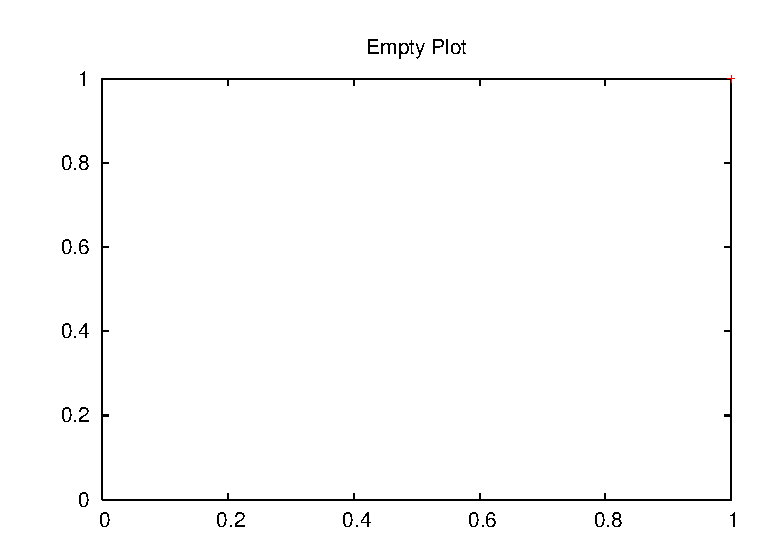
\includegraphics[height=1in]{F/empty.eps}
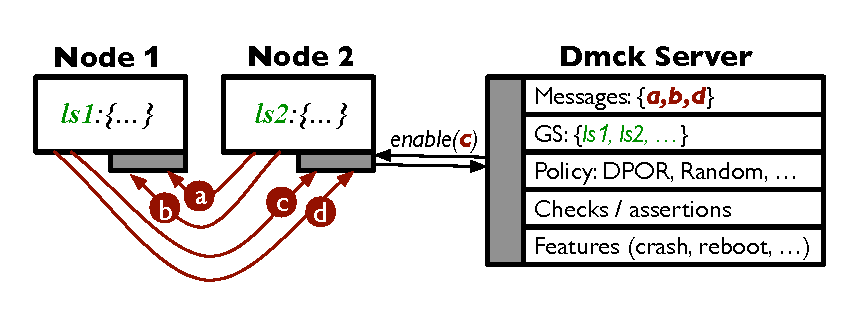
\includegraphics[height=2in]{F/dmck/dmck.eps}
}
\vminfive
\mycaption[Distributed System Model Checker]{fig-dmck}{DMCK}{The figure illustrates a typical framework
of a distributed system model checker (dmck).
}
%\vminten
\end{figure}

\if 0
The figure shows a dmck server model checking
a target distributed system containing two nodes.  
Communications in the target system are interposed 
\fi



The last ten years have seen a rise of software model checker that checks
distributed systems directly at the implementation level.  Figure~\ref{fig-dmck}
illustrates a dmck integration to a target distributed system, a simple
representation of existing dmck frameworks~\cite{Guo+11-Demeter,
Killian+07-LifeDeathMaceMC, Simsa+10-Dbug, Yang+09-Modist}.  The dmck inserts an
interposition layer in each node of the target system with the purpose of
controlling all important events (\eg, network messages, timeouts) and
preventing the target system to process the events until the dmck enables them.
A main dmck mechanism is the permutation of events; the goal is to push the
target system into all possible ordering scenarios.  For example, the dmck can
enforce \ts{abcd} ordering in one execution, \ts{bcad} in another, and so on.

\if 0 

\subsection{State-of-the-Art DMCKs}

\modist~\cite{Yang+09-Modist} is arguably one of the most powerful
dmcks that comes with systematic reduction policies.  \modist\ has been
integrated to real systems due to its exploration
scalability.  At the heart of \modist\ is {\em dynamic partial order
  reduction (DPOR)}~\cite{Flanagan+05-Dpor} which exploits the {\em
  independence} of events to reduce the state explosion.  Independent
events mean that it does not matter in what order the system execute
the events, as their different orderings are considered equivalent.

To illustrate how \modist\ adopts DPOR, let's use the example in
Figure~\ref{fig-dmck}, which shows four concurrent 
outstanding messages \ts{abcd}
(\ma\ and \mb\ for \none, \mc\ and \md\ for \ntwo).  A brute-force
approach will try all possible combinations (\ts{abcd}, \ts{abdc},
\ts{acbd}, \ts{acdb}, \ts{cabd}, and so on), for a total of 4!
executions.
% dpor
Fortunately, the notion of event independence can be mapped to
distributed system properties.  For example, \modist\ specifies this
reduction policy: a message to be processed by a given node is
independent of other concurrent messages destined to other nodes
(based on vector clocks).  Applying this policy to the example in
Figure~\ref{fig-dmck} implies that \ma\ and \mb\ are
dependent\footnote[1]{In model checking, ``dependent'' events mean
  that they must be re-ordered.  ``Dependent'' does not mean
  ``causally dependent''.}  but they are independent of \mc\ and
\md\ (and vice versa).  Since only dependent events need to be
reordered, this reduction policy leads to only 4 executions
(\ma\mb-\mc\md, \ma\mb-\md\mc, \mb\ma-\mc\md, \mb\ma-\md\mc), giving a
6x speed-up (4!/4).

Although \modist's speed-up is significant, we find that one 
scalability limitation of its DPOR application is within its {\em
  black-box} approach; it only exploits general properties of
distributed systems to define message independence.  It does not
exploit any semantic information from the target system to define more
independent events.  

% demeter
Dynamic interface reduction (DIR)~\cite{Guo+11-Demeter} is the next
advancement to \modist.  This work suggests that a complete dmck must
re-order not only messages (global events) but also thread
interleavings (local events).  The reduction intuition behind DIR is
that different thread interleavings often lead to the same global
events (\eg, a node sends the same messages regardless of how threads are
interleaved in that node).  DIR records local exploration and replays
future incoming messages without the need for global exploration.
In our work, SAMC focuses only on global exploration (message and fault
re-orderings).  We believe DIR is orthogonal to SAMC, similar to the
way DIR is orthogonal to \modist.

% besides (quick take)
\modist\ and DIR are examples of dmcks that employ advanced systematic
reduction policies.  LMC~\cite{Guerraoui+11-McNoNetwork} is similar to
DIR; it also decouples local and global exploration.
dBug~\cite{Simsa+10-Dbug} applies DPOR similarly to \modist.  There are
other dmcks such as \macemc~\cite{Killian+07-LifeDeathMaceMC} and
CrystalBall~\cite{Yabandeh+09-CrystalBall} that use basic exploration
methods such as depth first (DFS), weight-based,
and random searches.

% symmetry
Other than the aforementioned methods, {\em symmetry} is another
foundational reduction policy~\cite{Emerson+97-PorAndSym,
  Prasad+00-SymBasedMc}.  Symmetry-based methods exploit the
architectural symmetry present in the target system.  For example, in
a ring of nodes, one can rotate the ring without affecting
the behavior of the system.  Symmetry is powerful, but
we find no existing dmcks that adopt symmetry.

% multiple failures
Besides dmcks, there exists sophisticated testing frameworks for
distributed systems (\eg, \fate~\cite{Gunawi+11-FateDestini},
\prefail~\cite{Joshi+11-PreFail},
\setsudo~\cite{Joshi+13-SetsudoTesting}, OpenStack
fault-injector~\cite{Ju+13-FaultResOpenStack}). This set of work
emphasizes the importance of multiple faults, but their major
limitation is that they are not a dmck.  That is, they cannot
systematically control and permute non-deterministic choices such as
message and fault reorderings.

\fi
